\begin{titlepage}

\begin{center}


% Oberer Teil der Titelseite:
\hspace{2cm}
\vspace{2cm}
\begin{figure}[h!]
    \begin{minipage}[t]{0.4\textwidth}\vspace{0pt}
        \centering
        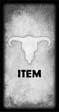
\includegraphics[width=2cm]{resources/item2}
    \end{minipage}\hfill%
    \begin{minipage}[t]{0.2\textwidth}\vspace{0pt}
        \centering
        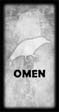
\includegraphics[width=2cm]{resources/omen2}
    \end{minipage}\hfill%
    \begin{minipage}[t]{0.4\textwidth}\vspace{0pt}
        \centering
        
\includegraphics[width=2cm]{resources/event2}
    \end{minipage}\hfill%
\end{figure}

\\[1.5cm]

\textsc{\LARGE Betrayal at House on the Hill}\\[0.5cm]

\textsc{A Strategy Game by B.G. - 2nd Edition}\\[1.5cm]

\textsc{\Large Deutsche Übersetzung}\\[0.5cm]



\HRule \\[1.5cm]

% Author and supervisor
\begin{minipage}{0.4\textwidth}
\begin{flushleft} \large
\emph{Autoren}\\
\\[0.3cm]
Fleißige \textsc{Mutanten}\\
Rothaarige \textsc{Hexen}\\
Lederhäutige \textsc{Höhlenbewohner}
\\[1.5cm]
\emph{Du willst mithelfen? / Download}
\\[0.3cm]
\url{https://github.com/maxTheOger/betrayal\_2ndedition\_german}\\
\\[1.5cm]
\emph{Dies ist die Version vom}
\\[0.3cm]
{\large \today}


\end{flushleft}
\end{minipage}
\hfill
\begin{minipage}{0.4\textwidth}
\begin{flushright} \large
\emph{Inhalt} \\
\\[0.3cm]
Regeln \\
Räume \\
Karten \\
Hauntchart \\
Secrets of Survival \\
Traitors Tome \\
\\[1.5cm]
\emph{Überarbeitete Übersetzungen}\\
\\[0.3cm]
Szenarien 1-2, 13
\end{flushright}
\end{minipage}

\vfill

% Unterer Teil der Seite
{\emph{Auf ins Abenteuer …}}

\end{center}

\end{titlepage}